% This file was created by tikzplotlib v0.9.1.
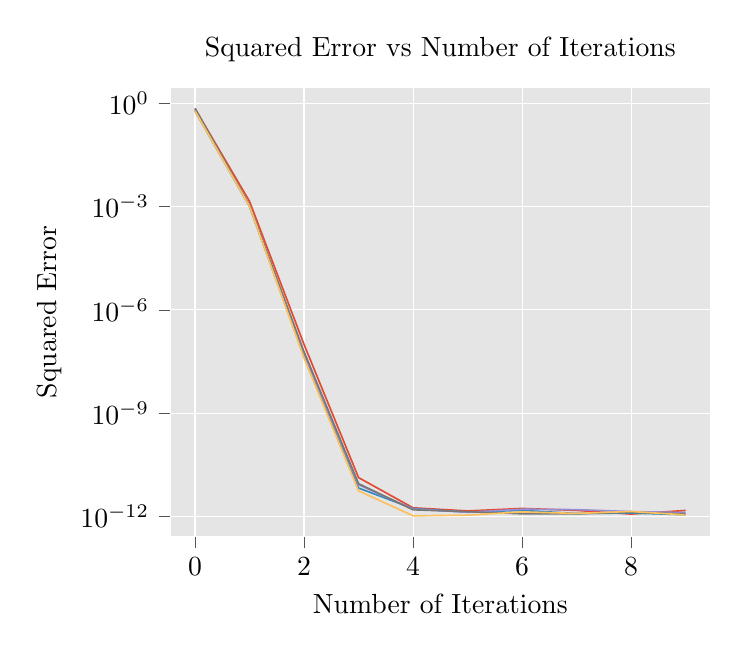
\begin{tikzpicture}

\definecolor{color0}{rgb}{0.886274509803922,0.290196078431373,0.2}
\definecolor{color1}{rgb}{0.203921568627451,0.541176470588235,0.741176470588235}
\definecolor{color2}{rgb}{0.596078431372549,0.556862745098039,0.835294117647059}
\definecolor{color3}{rgb}{0.984313725490196,0.756862745098039,0.368627450980392}

\begin{axis}[
axis background/.style={fill=white!89.8039215686275!black},
axis line style={white},
log basis y={10},
tick align=outside,
tick pos=left,
title={Squared Error vs Number of Iterations},
x grid style={white},
xlabel={Number of Iterations},
xlabel near ticks,
xmajorgrids,
xmin=-0.45, xmax=9.45,
xtick style={color=white!33.3333333333333!black},
y grid style={white},
ylabel={Squared Error},
ylabel near ticks,
ymajorgrids,
ymin=2.71273553797183e-13, ymax=2.77667975831396,
ymode=log,
ytick style={color=white!33.3333333333333!black}
]
\addplot [semithick, color0]
table {%
0 0.691431879997253
1 0.00141645281109959
2 9.95126896441434e-08
3 1.36033406761271e-11
4 1.80833126250945e-12
5 1.46727074934461e-12
6 1.73372427525464e-12
7 1.52411416820541e-12
8 1.19015908239817e-12
9 1.51345602716901e-12
};
\addplot [semithick, color1]
table {%
0 0.591166257858276
1 0.0010115496115759
2 4.45605756738132e-08
3 6.77857769915136e-12
4 1.71951342053944e-12
5 1.35713662530179e-12
6 1.52411416820541e-12
7 1.23634436022257e-12
8 1.27897692436818e-12
9 1.13686837721616e-12
};
\addplot [semithick, color2]
table {%
0 0.625002205371857
1 0.00102552131284028
2 5.11129663038901e-08
3 8.41993141875719e-12
4 1.66622271535743e-12
5 1.34292577058659e-12
6 1.64490643328463e-12
7 1.60227386913903e-12
8 1.406874616805e-12
9 1.31450406115619e-12
};
\addplot [semithick, white!46.6666666666667!black]
table {%
0 0.711470305919647
1 0.00108080555219203
2 6.08989694228512e-08
3 9.08784159037168e-12
4 1.58451030074502e-12
5 1.3962164757686e-12
6 1.21147536447097e-12
7 1.21147536447097e-12
8 1.33937305690779e-12
9 1.20792265079217e-12
};
\addplot [semithick, color3]
table {%
0 0.590315997600555
1 0.00102019123733044
2 3.97954451614169e-08
3 5.62394575354119e-12
4 1.05870867628255e-12
5 1.10844666778576e-12
6 1.37845290737459e-12
7 1.24344978758018e-12
8 1.4175327578414e-12
9 1.12265752250096e-12
};
\end{axis}

\end{tikzpicture}
